\documentclass{article}
\usepackage{listings}
\usepackage{xcolor}
\usepackage{enumitem}
\usepackage{graphicx}
\usepackage{amssymb}
\usepackage{bytefield}
\usepackage{forest}
\usepackage{float}
\usepackage{fancyhdr} % Custom headers/footers
\usepackage{colortbl}
\usepackage[left=0.6in, right=0.6in, top=1in, bottom=0.9in]{geometry}
\usepackage{indentfirst}
\usepackage{multicol}
\usepackage{multirow}
\usepackage{tikz}
\usetikzlibrary{automata, positioning}
\usepackage{changepage, titlesec}
\usepackage{booktabs}
\usepackage{array}
\usepackage{adjustbox} % for adjustwidth
\usepackage{multicol} % for side-by-side columns
\setlength{\parindent}{1.5em} % Set indentation size (optional)
\usepackage{amsmath} % Required for align environment
\usepackage{xepersian}
\settextfont{Vazirmatn FD}
\setlatintextfont{Noto Serif} 


\pagestyle{fancy}     % Enable fancy headers
\fancyhf{}            % Clear default header/footer
\renewcommand{\headrulewidth}{0pt} % Disable default header line

\fancyhead[L]{\rule{\textwidth}{1pt}} % Manually add one line
\fancyfoot[C]{\thepage} % Page number in the center of the footer

\newcommand{\colorbitbox}[3]{%
	\rlap{\bitbox{#2}{\color{#1}\rule{\width}{\height}}}%
	\bitbox{#2}{#3}}
\definecolor{lightcyan}{rgb}{0.84,1,1}
\definecolor{lightgreen}{rgb}{0.64,1,0.71}
\definecolor{lightred}{rgb}{1,0.7,0.71}

\definecolor{codegreen}{rgb}{0,0.6,0}
\definecolor{codegray}{rgb}{0.5,0.5,0.5}
\definecolor{codepurple}{rgb}{0.58,0,0.82}
\definecolor{backcolour}{rgb}{0.95,0.95,0.92}

\lstdefinestyle{mystyle}{
	backgroundcolor=\color{backcolour},   
	commentstyle=\color{codegreen},
	keywordstyle=\color{magenta},
	numberstyle=\tiny\color{codegray},
	stringstyle=\color{codepurple},
	basicstyle=\ttfamily\footnotesize,
	breakatwhitespace=false,         
	breaklines=true,                 
	captionpos=b,                    
	keepspaces=true,                 
	numbers=left,                    
	numbersep=5pt,                  
	showspaces=false,                
	showstringspaces=false,
	showtabs=false,                  
	tabsize=2
}

\lstset{style=mystyle}

\ExplSyntaxOn
\NewDocumentCommand{\ReverseWords}{m}
{
	\seq_set_split:Nnn \l_tmpa_seq { ~ } { #1 } % Split words by spaces
	\seq_reverse:N \l_tmpa_seq % Reverse the order of words
	\seq_use:Nn \l_tmpa_seq { ~ } % Join words with spaces and output
}
\ExplSyntaxOff


\begin{document}
	\author{ مجتبی ملائی \\ ۴۰۱۳۱۳۸۳ }
	\title{ \huge { تکلیف دوم}}
	\date{}
	\maketitle
	
\section{}
\begin{enumerate}[label=\textbf{\Alph*)}]
	\item
	با بررسی در $S$ می‌بینیم که $ S \overset{+}{\Rightarrow} S\alpha $ وجود دارد.
	ابتدا در $S \rightarrow AbS$ قانون $A$ را با سمت راست آن جایگزین می‌کنیم:   
\[
\begin{aligned}
	S &\rightarrow SaS \mid SaAbS \mid BbS \\
	A &\rightarrow SaA \mid B \\
	B &\rightarrow bS \mid c
\end{aligned}
\]
سپس طبق قانون گفته شده در اسلاید داریم:
\[
\begin{aligned}
	S &\rightarrow BbSS' \\
	S' &\rightarrow aSS' \mid aAbSS' \mid \epsilon \\
	A &\rightarrow SaA \mid B \\
	B &\rightarrow bS \mid c
\end{aligned}
\]

\item 
برای ساده سازی ابتدا $B$ و $C$ را جایگزین می‌کنیم.
\[
\begin{aligned}
	S &\rightarrow abcA \mid abcb \mid abc \\
	A &\rightarrow abA \mid abbA \mid abbc 
\end{aligned}
\]
سپس $abc$ را در $S$ فاکتور می‌گیریم.

\[
\begin{aligned}
	S &\rightarrow abcS' \\
	S' &\rightarrow A \mid b \mid \epsilon \\
	A &\rightarrow abA \mid abbA \mid abbc 
\end{aligned}
\]
در $A$ حروف $ab$ را فاکتور می‌گیریم.
 
\[
\begin{aligned}
	S &\rightarrow abcS' \\
	S' &\rightarrow A \mid b \mid \epsilon \\
	A &\rightarrow abA'\\
	A' &\rightarrow A \mid bA \mid bc 
\end{aligned}
\]
حال می‌توانیم دوباره $b$ را فاکتور بگیریم.

\[
\begin{aligned}
	S &\rightarrow abcS' \\
	S' &\rightarrow A \mid b \mid \epsilon \\
	A &\rightarrow abA' \\
	A' & \rightarrow A \mid bA'' \\ 
	A'' &\rightarrow  A \mid c 
\end{aligned}
\]


\end{enumerate}	
	
\section{} 
\begin{latin}
	\begin{table}[H]
		\centering
		\renewcommand{\arraystretch}{1.3} % Adjust row height
		\begin{tabular}{|c|c|c|}
			\hline
			\textbf{Non-terminals} & \textbf{First} & \textbf{Follow} \\
			\hline
			Program & \{ & \$ \\
			Statements & id , if , $\epsilon$ & \} \\
			Statement & id , if & id , if , \} \\
			Expression & id & ; , ) \\
			Tail & + , - , $\epsilon$ & ; , ) \\
			\hline
		\end{tabular}
		\caption{First and Follow sets for non-terminals}
		\label{tab:first_follow}
	\end{table}

\begin{lstlisting}[language=C, caption=Recursive Descent Parser Pseudo-Code]
// Assume we have a function `nextToken()` that gets the next token from the input stream
// Assume `currentToken` holds the current token
// Assume `match(expected)` matches the current token and advances to the next one
function Program():
	if currentToken == '{':
		match('{')
		Statements()
		match('}')
		match('eof') // Ensure the program ends correctly
	else:
		error("Expected '{' at the start of the program")
			
function Statements():
	if currentToken in {'id', 'if'}: // FIRST(Statements)
		Statement()
		Statements()
		else:
			// epsilon (FOLLOW(Statements) is { '}' }), so we return without consuming anything
function Statement():
	if currentToken == 'id':
		match('id')
		match('=')
		Expression()
		match(';')
	else if currentToken == 'if':
		match('if')
		match('(')
		Expression()
		match(')')
		Statement()
	else:
		error("Invalid statement")
		
function Expression():
	if currentToken == 'id':
		match('id')
		Tail()
	else:
		error("Expected identifier in expression")
		
function Tail():
	if currentToken == '+':
		match('+')
		Expression()
	else if currentToken == '-':
		match('-')
		Expression()
	else:
		// epsilon (FOLLOW(Tail) is { ';' , ')' }), so we return without consuming anything
\end{lstlisting}
\end{latin}	
	
\section{}

\begin{enumerate}
	\item   ‎  
	 \begin{latin}
		\begin{table}[H]
			\centering
			\renewcommand{\arraystretch}{1.3} % Adjust row height
			\begin{tabular}{|c|c|c|}
				\hline
				\textbf{Non-terminals} & \textbf{First} & \textbf{Follow} \\
				\hline
				S & if & \$ \\
				\hline
				I & =, $\epsilon$ & \$ \\
				\hline
				E & (, id, num & \$, ), then  \\
				\hline
				E'& + , $\epsilon$ &  \$, ), then  \\
				\hline 
				T & (, id, num & +, \$, ), then \\
				\hline 
				T'& *, $\epsilon$  &  +, \$, ), then  \\
				\hline 
				F &  (, id, num & *, +, \$, ), then  \\
				\hline
			\end{tabular}
			\label{tab:first_follow2}
		\end{table}
	\end{latin}
	\item   ‎  
	\begin{latin}
		\centering
		\begin{tabular}{|c|c|c|c|c|c|c|c|c|c|c|}
			
			\hline
			
& $id$ & $num$ & $($ & $)$ & $+$ & $*$ &$=$&$if$& $then$ & $\$$ \\
			\hline
$S$ & $idI$ &  &  &  &  &  &  & $if E then S$ &  &  \\
			\hline
$I$ &  &  &  &  &  &  &  &  &  & $e$ \\
			\hline
$E$ & $TE'$ & $TE'$ & $TE'$ &  &  &  &  &  &  &  \\
			\hline
$E'$&  &  &  &$\epsilon$ &$+TE'$  &  &  &  & $\epsilon$ & $\epsilon$ \\
			\hline
$T$ & $FT'$ & $FT'$ & $FT'$ &  &  &  &  &  &  &  \\
			\hline
$T'$ &  &  &  & $\epsilon$ & $\epsilon$ & $*FT'$  &  &  & $\epsilon$ & $\epsilon$  \\
			\hline
$F$ & $id$  &$num$  & $(E)$  &  &  &  &  &  &  &  \\
			\hline
			
		\end{tabular}
		
	\end{latin}
	
	\item  ‎  
\begin{latin}
\begin{table}[H]
	\centering
	\renewcommand{\arraystretch}{1.3}
	\resizebox{\textwidth}{!}{%
		\begin{tabular}{|c|l|l|l|l|}
			\hline 
			\textbf{Step} & \textbf{Matched} & \textbf{Stack} & \textbf{Input} & \textbf{Action} \\
			\hline  			
			1  & $\epsilon$             & $S$                         & $if\ id\ then\ id\ =\ (\,num\,*\,id\,)\ +\ num\ \$ $ &  \\
			2  & $\epsilon$             & $if\ E\ then\ S$            & $if\ id\ then\ id\ =\ (\,num\,*\,id\,)\ +\ num\ \$ $ & output $S \rightarrow if\ E\ then\ S$ \\
			3  & $if$                   & $E\ then\ S$                & $id\ then\ id\ =\ (\,num\,*\,id\,)\ +\ num\ \$ $ & match $if$ \\
			4  & $if$                   & $T\ E'\ then\ S$            & $id\ then\ id\ =\ (\,num\,*\,id\,)\ +\ num\ \$ $ & output $E \rightarrow T\ E'$ \\
			5  & $if$                   & $F\ T'\ E'\ then\ S$        & $id\ then\ id\ =\ (\,num\,*\,id\,)\ +\ num\ \$ $ & output $T \rightarrow F\ T'$ \\
			6  & $if$                   & $id\ T'\ E'\ then\ S$       & $id\ then\ id\ =\ (\,num\,*\,id\,)\ +\ num\ \$ $ & output $F \rightarrow id$ \\
			7  & $if\ id$               & $T'\ E'\ then\ S$           & $then\ id\ =\ (\,num\,*\,id\,)\ +\ num\ \$ $ & match $id$ \\
			8  & $if\ id$               & $E'\ then\ S$               & $then\ id\ =\ (\,num\,*\,id\,)\ +\ num\ \$ $ & output $T' \rightarrow \epsilon$ \\
			9  & $if\ id$               & $then\ S$                   & $then\ id\ =\ (\,num\,*\,id\,)\ +\ num\ \$ $ & output $E' \rightarrow \epsilon$ \\
			10 & $if\ id\ then$         & $S$                         & $id\ =\ (\,num\,*\,id\,)\ +\ num\ \$ $ & match $then$ \\
			11 & $if\ id\ then$         & $id\ I$                     & $id\ =\ (\,num\,*\,id\,)\ +\ num\ \$ $ & output $S \rightarrow id\ I$ \\
			12 & $if\ id\ then\ id$     & $I$                         & $=\ (\,num\,*\,id\,)\ +\ num\ \$ $ & match $id$ \\
			13 & $if\ id\ then\ id$     & $=\ E$                      & $=\ (\,num\,*\,id\,)\ +\ num\ \$ $ & output $I \rightarrow =\ E$ \\
			14 & $if\ id\ then\ id\ =$  & $E$                         & $(\,num\,*\,id\,)\ +\ num\ \$ $ & match $=$ \\
			15 & $if\ id\ then\ id\ =$  & $T\ E'$                     & $(\,num\,*\,id\,)\ +\ num\ \$ $ & output $E \rightarrow T\ E'$ \\
			16 & $if\ id\ then\ id\ =$  & $F\ T'\ E'$                 & $(\,num\,*\,id\,)\ +\ num\ \$ $ & output $T \rightarrow F\ T'$ \\
			17 & $if\ id\ then\ id\ =$  & $(\ E\ )\ T'\ E'$           & $(\,num\,*\,id\,)\ +\ num\ \$ $ & output $F \rightarrow (E)$ \\
			18 & $if\ id\ then\ id\ =($ & $E\ )\ T'\ E'$              & $num\,*\,id\,)\ +\ num\ \$ $ & match $($ \\
			19 & $if\ id\ then\ id\ =($ & $T\ E'\ )\ T'\ E'$          & $num\,*\,id\,)\ +\ num\ \$ $ & output $E \rightarrow T\ E'$ \\
			20 & $if\ id\ then\ id\ =($ & $F\ T'\ E'\ )\ T'\ E'$      & $num\,*\,id\,)\ +\ num\ \$ $ & output $T \rightarrow F\ T'$ \\
			21 & $if\ id\ then\ id\ =($ & $num\ T'\ E'\ )\ T'\ E'$    & $num\,*\,id\,)\ +\ num\ \$ $ & output $F \rightarrow num$ \\
			22 & $if\ id\ then\ id\ =(\ num$ & $T'\ E'\ )\ T'\ E'$    & $*\,id\,)\ +\ num\ \$ $ & match $num$ \\
			23 & $if\ id\ then\ id\ =(\ num$ & $*\ F\ T'\ E'\ )\ T'\ E'$ & $id\,)\ +\ num\ \$ $ & output $T' \rightarrow *\ F\ T'$ \\
			24 & $if\ id\ then\ id\ =(\ num\ *$ & $F\ T'\ E'\ )\ T'\ E'$ & $id\,)\ +\ num\ \$ $ & match $*$ \\
			25 & $if\ id\ then\ id\ =(\ num\ *$ & $id\ T'\ E'\ )\ T'\ E'$ & $id\,)\ +\ num\ \$ $ & output $F \rightarrow id$ \\
			26 & $if\ id\ then\ id\ =(\ num\ *\ id$ & $T'\ E'\ )\ T'\ E'$ & $)\ +\ num\ \$ $ & match $id$ \\
			27 & $if\ id\ then\ id\ =(\ num\ *\ id$ & $E'\ )\ T'\ E'$ & $)\ +\ num\ \$ $ & output $T' \rightarrow \epsilon$ \\
			28 & $if\ id\ then\ id\ =(\ num\ *\ id$ & $)\ T'\ E'$     & $)\ +\ num\ \$ $ & output $E' \rightarrow \epsilon$ \\
			29 & $if\ id\ then\ id\ =(\ num\ *\ id\ )$ & $T'\ E'$     & $+\ num\ \$ $ & match $)$ \\
			30 & $if\ id\ then\ id\ =(\ num\ *\ id\ )$ & $+\ T\ E'$   & $num\ \$ $ & output $E' \rightarrow + T E'$ \\
			31 & $if\ id\ then\ id\ =(\ num\ *\ id\ )\ +$ & $T\ E'$   & $num\ \$ $ & match $+$ \\
			32 & $if\ id\ then\ id\ =(\ num\ *\ id\ )\ +$ & $F\ T'\ E'$ & $num\ \$ $ & output $T \rightarrow F T'$ \\
			33 & $if\ id\ then\ id\ =(\ num\ *\ id\ )\ +$ & $num\ T'\ E'$ & $num\ \$ $ & output $F \rightarrow num$ \\
			34 & $if\ id\ then\ id\ =(\ num\ *\ id\ )\ +\ num$ & $T'\ E'$ & \$ & match $num$ \\
			35 & $if\ id\ then\ id\ =(\ num\ *\ id\ )\ +\ num$ & $E'$  & \$ & output $T' \rightarrow \epsilon$ \\
			36 & $if\ id\ then\ id\ =(\ num\ *\ id\ )\ +\ num$ &        & \$ & output $E' \rightarrow \epsilon$ \\
			37 & $if\ id\ then\ id\ =(\ num\ *\ id\ )\ +\ num\ \$ $ &   & & match \$ \\
			\hline
		\end{tabular}
	}
	\caption{LL(1) Parsing Trace for \texttt{if id then id = ( num * id ) + num}}
\end{table}

\end{latin}


\end{enumerate}



\section{}

\begin{enumerate}
	\item 
	ابتدا فاکتور گیری چپ انجام می‌دهیم.
	 \begin{latin}
	 	$S \rightarrow iEtSA | a $ \\ 
	 	$A \rightarrow \epsilon | eS $ \\ 
	 	$E \rightarrow B$\\
	 \end{latin}

	\vspace{2cm}
	
	سپس گرامر را به فرم مورد نیاز تبدیل می‌کنیم
	\begin{latin}
		$0: \space S' \rightarrow S$ \\
		$1: \space S \rightarrow iEtSA$ \\ 
		$2: \space S \rightarrow a$ \\ 
		$3: \space A \rightarrow eS $ \\
		$4:\space A \rightarrow \epsilon $ \\ 
		$5: \space E \rightarrow b$ \\
	\end{latin}

\begin{latin}
	\begin{minipage}[t]{0.19\linewidth}
		$I_0:$ \\
		\(
		S'\rightarrow .S\$ \\
		S \rightarrow .iEtSA \\
		S \rightarrow .a \\
		\)
	\end{minipage}
	\begin{minipage}[t]{0.19\linewidth}
		$I_1:$ \\
		\(
		S'\rightarrow S.\$ \\
		\)
	\end{minipage}
	\begin{minipage}[t]{0.19\linewidth}
		$I_2:$ \\
		\(
		S \rightarrow a. \\
		\)
	\end{minipage}
	\begin{minipage}[t]{0.19\linewidth}
		$I_3:$ \\
		\(
		S \rightarrow i.EtSA \\
		E \rightarrow .b
		\)
	\end{minipage}
	\begin{minipage}[t]{0.19\linewidth}
		$I_4:$ \\
		\(
		E \rightarrow b.
		\)
	\end{minipage}
		\begin{minipage}[t]{0.2\linewidth}
		$I_5:$ \\
		\(
		S \rightarrow iE.tSA \\
		\)
	\end{minipage}
	\begin{minipage}[t]{0.2\linewidth}
		$I_6:$ \\
		\(	
		S \rightarrow .iEt.SA \\
		S \rightarrow .iEtSA \\
		S \rightarrow .a \\
		\)
	\end{minipage}
	\begin{minipage}[t]{0.2\linewidth}
		$I_7:$ \\
		\(
		S \rightarrow iEtS.A \\
		A \rightarrow . \\
		A \rightarrow eS \\
		\)
	\end{minipage}
	\begin{minipage}[t]{0.2\linewidth}
		$I_8:$ \\
		\(
		S \rightarrow iEtSA. \\
		\)
	\end{minipage}
	\begin{minipage}[t]{0.2\linewidth}
		$I_{9}:$ \\
		\(
		A \rightarrow e.S\\
		S \rightarrow .iEtSA \\
		S \rightarrow .a \\
		\)
	\end{minipage}
	\begin{minipage}[t]{0.2\linewidth}
		$I_{10}:$ \\
		\(
		A \rightarrow eS.
		\)
	\end{minipage}
\end{latin}	

\begin{latin}
	\centering
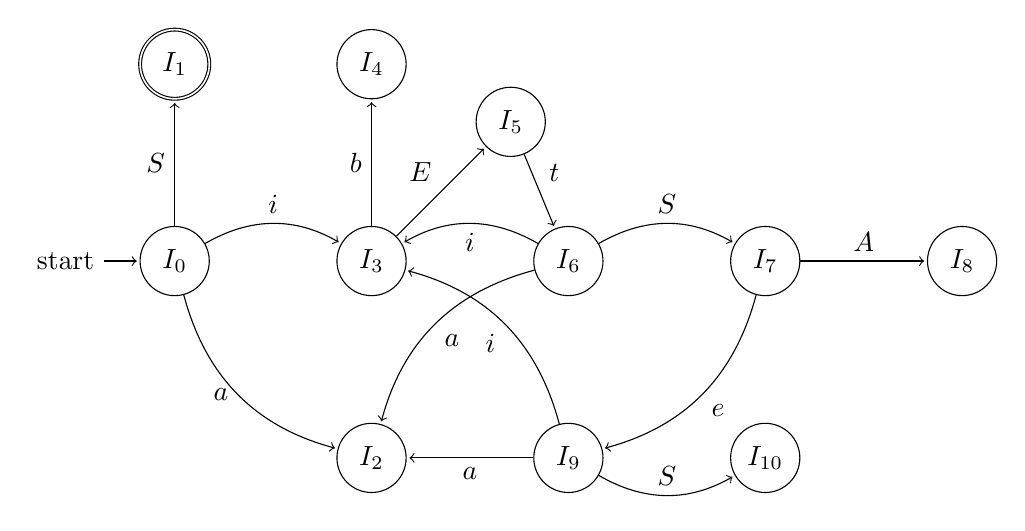
\begin{tikzpicture}[shorten >=1pt, node distance=2.5cm, on grid, auto] 
	\node[state, initial] (i0)   {$I_0$}; 
	\node[state, accepting] (i1) [above=of i0] {$I_1$}; 
	\node[state] (i3) [right=of i0] {$I_3$}; 
	\node[state] (i2) [below=of i3] {$I_2$}; 
	\node[state] (i4) [above =of i3] {$I_4$};
	\node[state] (i5) [above right=of i3] {$I_5$}; 
	\node[state] (i6) [right=of i3] {$I_6$};
	\node[state] (i7) [right=of i6] {$I_7$};
	\node[state] (i8) [right=of i7]{$I_8$};
	\node[state] (i9) [below =of i6] {$I_9$};
	\node[state] (i10)[right=of i9] {$I_{10}$};
	\path[->] 
	(i0) edge[bend left] node {$i$} (i3)
	(i0) edge[bend right] node[left] {$a$} (i2)
	(i0) edge node {$S$} (i1)
	(i3) edge node {$b$} (i4)
	(i3) edge node {$E$} (i5)
	(i5) edge node {$t$} (i6)
	(i6) edge[bend right] node {$i$} (i3)
	(i6) edge[bend right] node {$a$} (i2)
	(i6) edge[bend left] node {$S$} (i7)
	(i7) edge node {$A$} (i8)
	(i7) edge[bend left] node {$e$} (i9)
	(i9) edge node {$a$} (i2)
	(i9) edge[bend right] node {$i$} (i3) 
	(i9) edge[bend right] node {$S$} (i10) 
	;
	
\end{tikzpicture}
\end{latin}
در $ّI_1$ با $\$$ به اکسپت می‌رویم. 
\item 
 ‎ 
\begin{latin}
	\centering
	\begin{tabular}{|c|c|c|c|c|c|c|c|c|c|}
		\hline
		 &\multicolumn{6}{c|}{\textbf{Action}} & \multicolumn{3}{c|}{\textbf{GOTO}} \\
		\hline
		 \textbf{state} & $a$ & $b$ & $e$ & $i$ & $t$& $\$$ &  $A$ & $E$ & $S$ \\
		\hline
		0&s2&&&s3&&&&&1 \\
		\hline 
		1&&&&&&acc&&& \\
		\hline 
		2&\multicolumn{6}{c|}{r2} &&& \\
		\hline
		3&&s4&&&&&&2& \\
		\hline 
		4&\multicolumn{6}{c|}{r5} &&& \\
		\hline 
		5&&&&&s5&&&& \\	
		\hline	
		6&s2&&&s3&&&&&7 \\
		\hline 		
		7&\multicolumn{2}{c|}{r4}&r4 \& s9&\multicolumn{3}{c|}{r4} &8&& \\
		\hline 
		8&\multicolumn{6}{c|}{r1} &&& \\
		\hline 
		9&s2&&&s3&&&&&10 \\
		\hline
		10&\multicolumn{6}{c|}{r3} &&& \\
		\hline 
	\end{tabular}
\end{latin} 
action های خالی به معنی error هستند!

در حالت ۷ برای \lr{\texttt{Action[7,$e$]}} هم reduce داریم و هم .shift بنابراین گرامر \lr{LR(0)} نیست.
\end{enumerate}


\section{}

\begin{enumerate}
	\item
	نیاز داریم گرامر را به شکل زیر تبدیل دهیم. 
	\begin{latin}
		\(
		0:\space S' \rightarrow S \\
		1:\space S \rightarrow i \\
		2:\space S \rightarrow SS+ \\
		3:\space S \rightarrow SS* \\
		\)
	\end{latin}
	
\begin{latin}
	\centering
	\begin{tabular}{|c|c|c|c|c|c|l|}
		\hline
		&  \multicolumn{4}{c|}{\texttt{ACTION}} & \texttt{GOTO} &    \\
		\hline 
		\textbf{state} & $+$  & $*$  & $i$  & $\$$  & $S$ & \textbf{Explanation} \\
		\hline
		0 &  &  & s1 &  & 2 & Initial state; shift on `i` to state 1, go to 2 on `S` \\
		\hline
		1 & \multicolumn{4}{c|}{r1} &  & Reduce using rule 1: \( S \rightarrow i \) \\
		\hline
		2 &  &  & s1 & acc & 3 & After first `S`; shift `i` to 1 or accept if input ends \\
		\hline
		3 & s4 & s5 & s1 &  & 3 & After `S`; can shift `+`, `*`, or another `i` \\
		\hline
		4 & \multicolumn{4}{c|}{r2} &  & Reduce using rule 2: \( S \rightarrow SS+ \) \\
		\hline
		5 & \multicolumn{4}{c|}{r3} &  & Reduce using rule 3: \( S \rightarrow SS* \) \\
		\hline
	\end{tabular}
\end{latin}

\item  ‎ 
\centering
\begin{latin}
	

\begin{tabular}{|c|c|c|c|c|}
	\hline
	step & stack  & input & handle &  action  \\
	\hline
	0 & $\$$  & $iii*i+*$ &  & shift  \\
	\hline
	1 & $\$i$  & $ii*i+*\$$ & $i$  & reduce  1 \\
\hline
	2 & $\$S$  & $ii*i+*\$$ &   & shift \\
\hline
	3 & $\$Si$  & $i*i+*\$$ & $i$  & reduce 1 \\
\hline
	4 & $\$SS$  & $i*i+*\$$ &   & shift \\
\hline
	5 & $\$SSi$  & $*i+*\$$ & $i$  & reduce 1 \\
\hline
	6 & $\$SSS$  & $*i+*\$$ &   & shift \\
\hline
	7 & $\$SSS*$  & $i+*\$$ & $SS*$  & reduce 3 \\
\hline
	8 & $\$SS$  & $i+*\$$ &   & shift \\
\hline
	9 & $\$SSi$  & $+*\$$ & $i$  & reduce 1 \\
\hline
	10 & $\$SSS$  & $+*\$$ &   & shift \\
\hline
	11 & $\$SSS+$  & $*\$$ & $SS+$  & reduce 2 \\
\hline
	12 & $\$SS$  & $*\$$ &   & shift \\
\hline
	13 & $\$SS*$  & $\$$ & $SS*$  & reduce 3 \\
\hline
	14 & $\$S$  & $\$$ &   & acc \\
\hline
\end{tabular}
\end{latin}
\end{enumerate}
\section{}
گرامر را به شکل زیر تبدیل می‌کنیم.
\begin{latin}
	\noindent~
	\(
		0: S' \rightarrow S \\
		1: S \rightarrow XdY \\
		2: X \rightarrow aX \\
		3: X \rightarrow \epsilon \\
		4: Y \rightarrow bYS \\
		5: Y \rightarrow \epsilon \\ 
	\)
\end{latin}
	حال در $I_0$ داریم: 

\begin{latin}
	\noindent
	\(
	0: S' \rightarrow .S \\
	1: S \rightarrow .XdY \\
	2: X \rightarrow .aX \\
	3: X \rightarrow . \\
	\)
\end{latin}
در این حالت چون نقطه به احر رسیده است یک reduce مربوط به $3: X \rightarrow  \epsilon$ همچنین یک شیفت داریم $2: X \rightarrow .aX$ بنابراین اگر جدول را بکشیم، در یکی از خانه ها collision رخ خواهد داد پس \lr{LR(0)} نیست.
\end{document}